\documentclass[11pt,a4paper]{report}
\usepackage[textwidth=37em,vmargin=30mm]{geometry}
\usepackage{calc,xunicode,amsmath,amssymb,paralist,enumitem,tabu,booktabs,datetime2,xeCJK,xeCJKfntef,listings}
\usepackage{tocloft,fancyhdr,tcolorbox,xcolor,graphicx,eso-pic,xltxtra,xelatexemoji}

\newcommand{\envyear}[0]{2025}
\newcommand{\envdatestr}[0]{2025-10-29}
\newcommand{\envfinaldir}[0]{webdb/2025/20251029/final}

\usepackage[hidelinks]{hyperref}
\hypersetup{
    colorlinks=false,
    pdfpagemode=FullScreen,
    pdftitle={Web Digest - \envdatestr}
}

\setlength{\cftbeforechapskip}{10pt}
\renewcommand{\cftchapfont}{\rmfamily\bfseries\large\raggedright}
\setlength{\cftbeforesecskip}{2pt}
\renewcommand{\cftsecfont}{\sffamily\small\raggedright}

\setdefaultleftmargin{2em}{2em}{1em}{1em}{1em}{1em}

\usepackage{xeCJK,xeCJKfntef}
\xeCJKsetup{PunctStyle=plain,RubberPunctSkip=false,CJKglue=\strut\hskip 0pt plus 0.1em minus 0.05em,CJKecglue=\strut\hskip 0.22em plus 0.2em}
\XeTeXlinebreaklocale "zh"
\XeTeXlinebreakskip = 0pt


\setmainfont{Brygada 1918}
\setromanfont{Brygada 1918}
\setsansfont{IBM Plex Sans}
\setmonofont{JetBrains Mono NL}
\setCJKmainfont{Noto Serif CJK SC}
\setCJKromanfont{Noto Serif CJK SC}
\setCJKsansfont{Noto Sans CJK SC}
\setCJKmonofont{Noto Sans CJK SC}

\setlength{\parindent}{0pt}
\setlength{\parskip}{8pt}
\linespread{1.15}

\lstset{
	basicstyle=\ttfamily\footnotesize,
	numbersep=5pt,
	backgroundcolor=\color{black!5},
	showspaces=false,
	showstringspaces=false,
	showtabs=false,
	tabsize=2,
	captionpos=b,
	breaklines=true,
	breakatwhitespace=true,
	breakautoindent=true,
	linewidth=\textwidth
}






\newcommand{\coverpic}[2]{
    % argv: itemurl, authorname
    Cover photo by #2~~(\href{#1}{#1})
}
\newcommand{\makeheader}[0]{
    \begin{titlepage}
        % \newgeometry{hmargin=15mm,tmargin=21mm,bmargin=12mm}
        \begin{center}
            
            \rmfamily\scshape
            \fontspec{BaskervilleF}
            \fontspec{Old Standard}
            \fontsize{59pt}{70pt}\selectfont
            WEB\hfill DIGEST
            
            \vfill
            % \vskip 30pt
            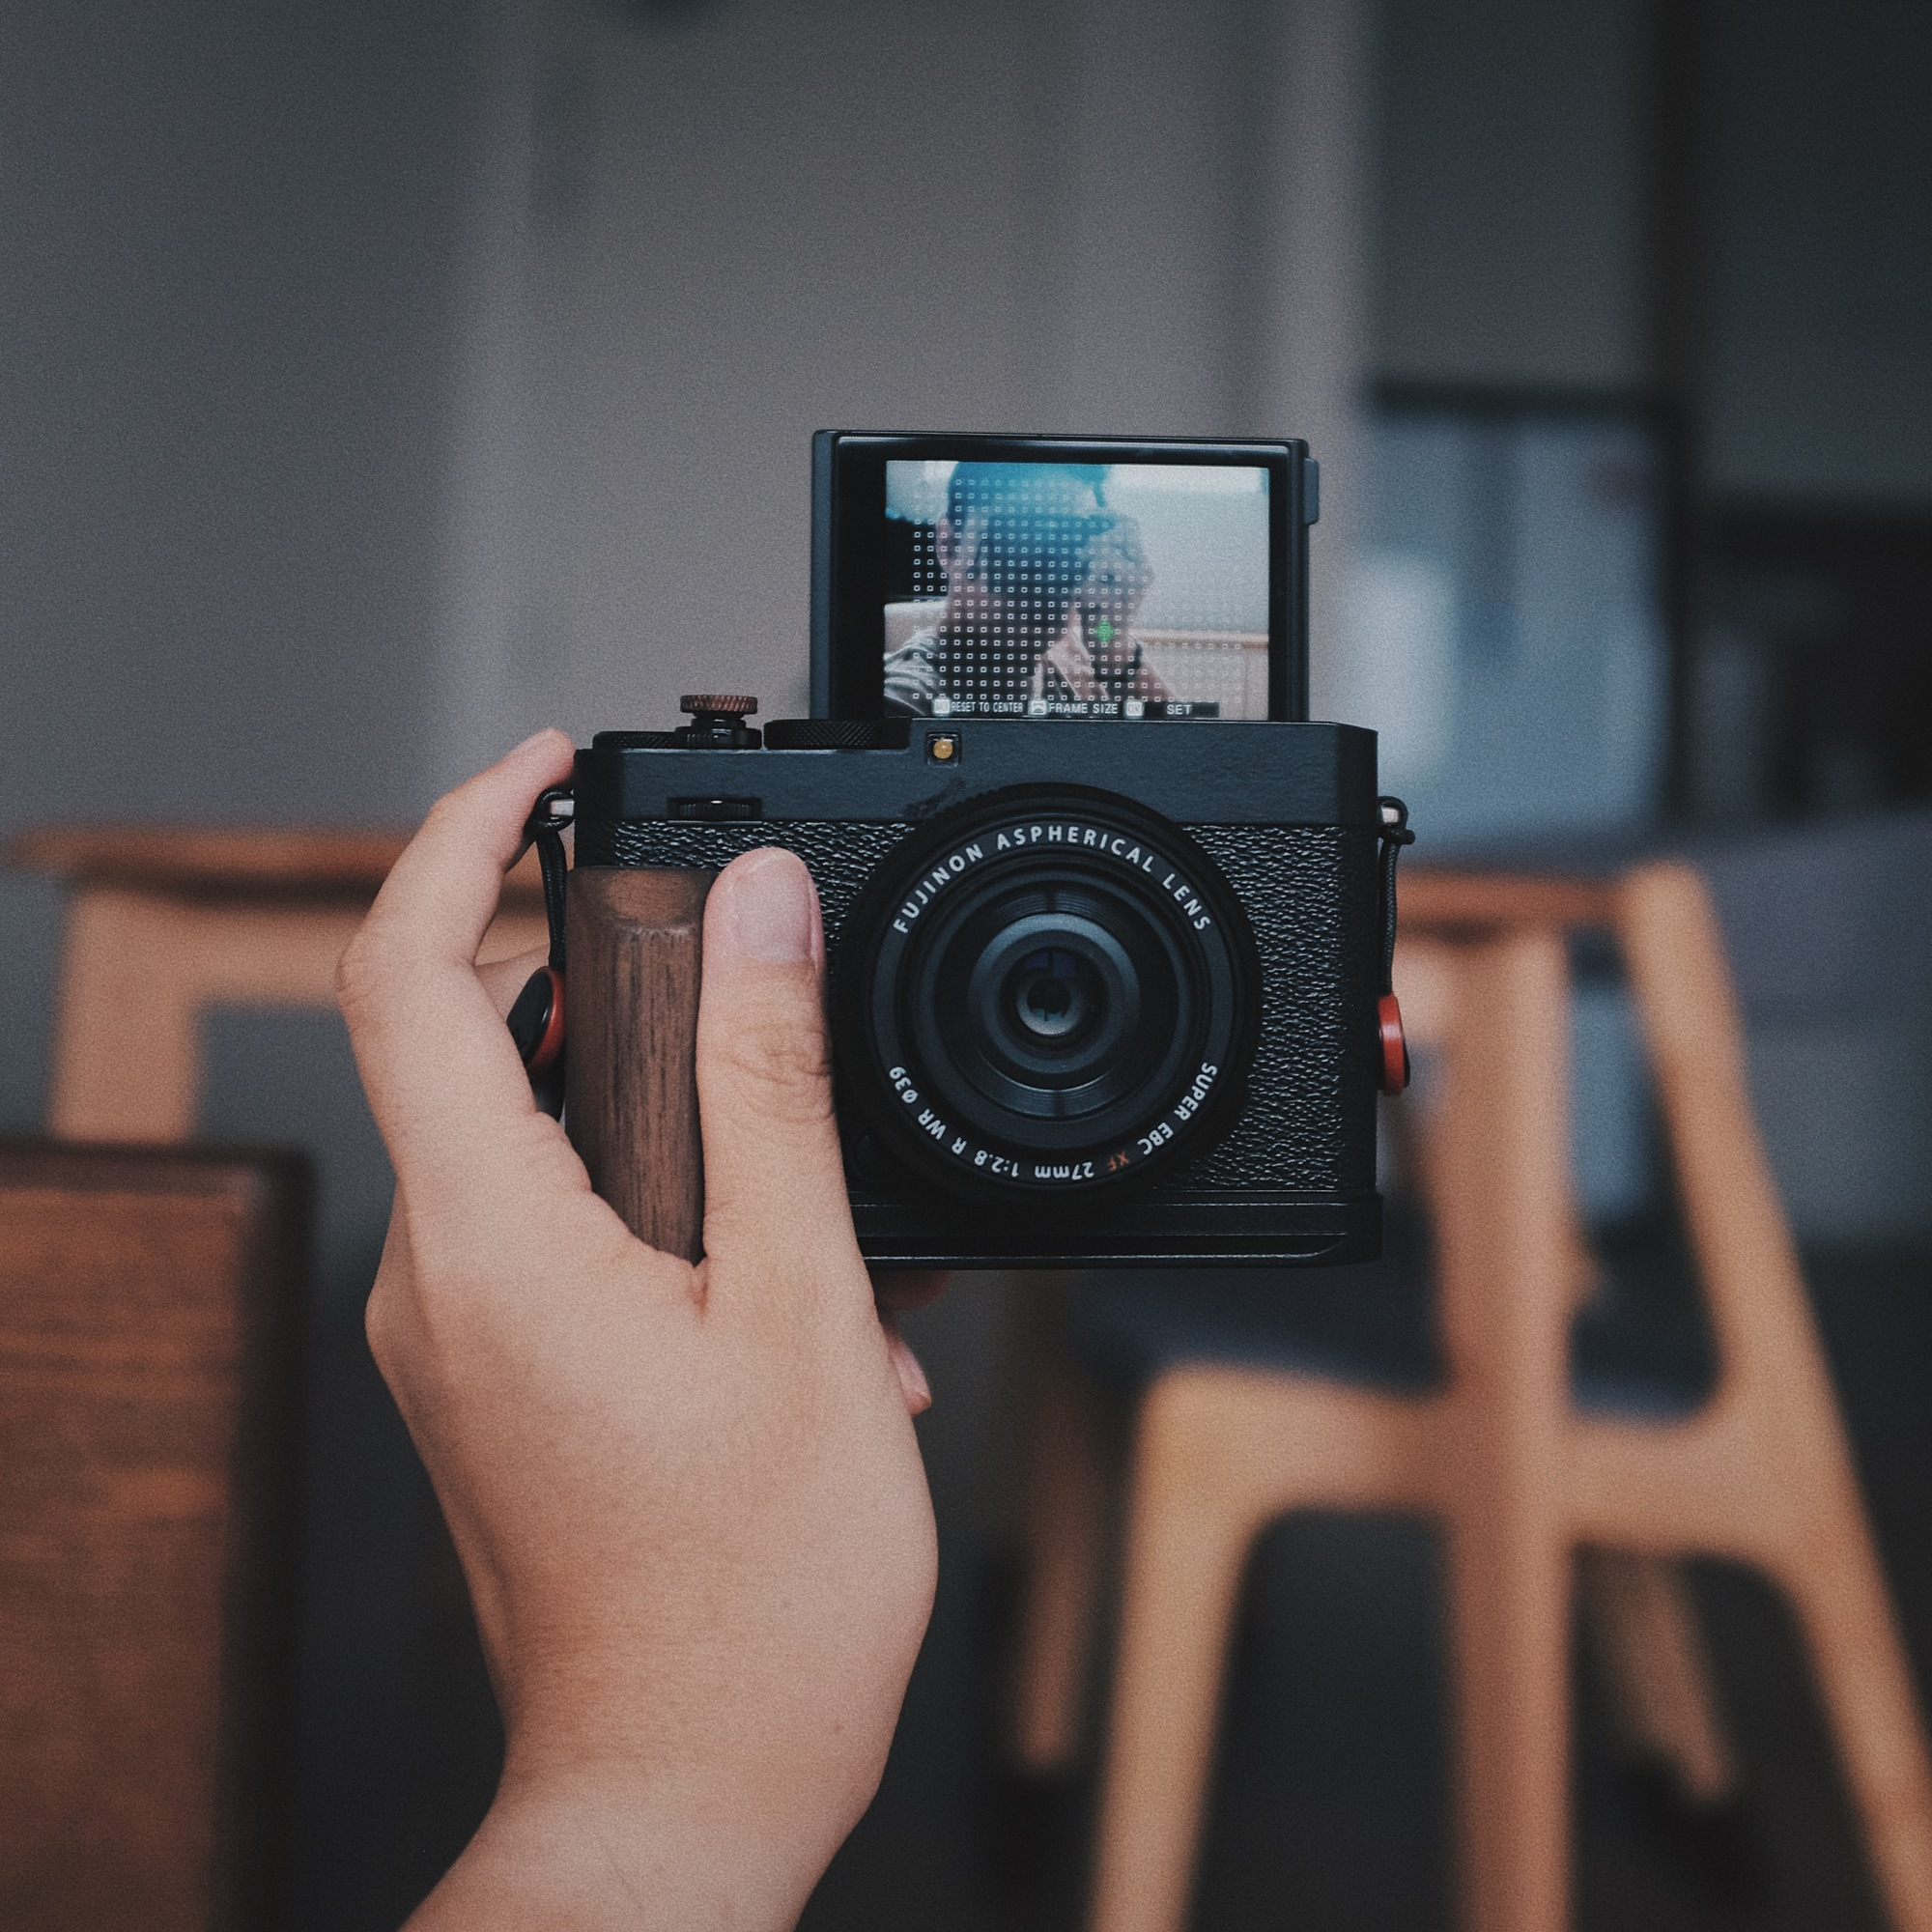
\includegraphics[width=\linewidth]{\envfinaldir/coverpic-prod.jpg}\par
            % \vskip 30pt
            \vfill

            \normalsize\rmfamily\scshape
            \copyright{} The Web Digest Project \hfill\large \envdatestr
        \end{center}
    \end{titlepage}
    % \restoregeometry
}
\newcommand{\simplehref}[1]{%
    \textcolor{blue!80!green}{\href{#1}{#1}}%
}
\renewcommand{\contentsname}{\center\Huge\sffamily\bfseries Contents\par\vskip 20pt}
\newcounter{ipartcounter}
\setcounter{ipartcounter}{0}
\newcommand{\ipart}[1]{
    % \vskip 20pt
    \clearpage
    \stepcounter{ipartcounter}
    \phantomsection
    \addcontentsline{toc}{chapter}{#1}
    % \begin{center}
    %     \Huge
    %     \sffamily\bfseries
    %     #1
    % \end{center}
    % \vskip 20pt plus 7pt
}
\newcounter{ichaptercounter}
\setcounter{ichaptercounter}{0}
\newcommand{\ichapter}[1]{
    % \vskip 20pt
    \clearpage
    \stepcounter{ichaptercounter}
    \phantomsection
    \addcontentsline{toc}{section}{\numberline{\arabic{ichaptercounter}}#1}
    \begin{center}
        \Huge
        \sffamily\bfseries
        #1
    \end{center}
    \vskip 20pt plus 7pt
}
\newcommand{\entrytitlefont}[1]{\subsection*{\raggedright\Large\sffamily\bfseries#1}}
\newcommand{\entryitemGeneric}[2]{
    % argv: title, url
    \parbox{\linewidth}{
        \entrytitlefont{#1}\par\vskip 5pt
        \footnotesize\ttfamily\mdseries
        \simplehref{#2}
    }\vskip 11pt plus 11pt minus 1pt
}
\newcommand{\entryitemGithub}[3]{
    % argv: title, url, desc
    \parbox{\linewidth}{
        \entrytitlefont{#1}\par\vskip 5pt
        \footnotesize\ttfamily\mdseries
        \simplehref{#2}\par\vskip 5pt
        \small\rmfamily\mdseries#3
    }\vskip 11pt plus 11pt minus 1pt
}
\newcommand{\entryitemAp}[3]{
    % argv: title, url, desc
    \parbox{\linewidth}{
        \entrytitlefont{#1}\par\vskip 5pt
        \footnotesize\ttfamily\mdseries
        \simplehref{#2}\par\vskip 5pt
        \small\rmfamily\mdseries#3
    }\vskip 11pt plus 11pt minus 1pt
}
\newcommand{\entryitemHackernews}[3]{
    % argv: title, hnurl, rawurl
    % \parbox{\linewidth}{
    %     \entrytitlefont{#1}\par\vskip 5pt
    %     \footnotesize\ttfamily\mdseries
    %     \simplehref{#3}\par
    %     \textcolor{black!50}{\href{#2}{#2}}
    % }\vskip 11pt plus 11pt minus 1pt
    \begin{minipage}{\linewidth}
            \entrytitlefont{#1}\par\vskip 5pt
            \footnotesize\ttfamily\mdseries
            \simplehref{#3}\par
            \textcolor{black!50}{\href{#2}{#2}}
    \end{minipage}\par\vskip 11pt plus 11pt minus 1pt
}







\begin{document}

\makeheader

\tableofcontents\clearpage




\ipart{Developers}
\ichapter{Hacker News}
\entryitemTwoLinks{Boring is what we wanted}{https://news.ycombinator.com/item?id=45738247}{https://512pixels.net/2025/10/boring-is-what-we-wanted/}

\entryitemTwoLinks{Samsung makes ads on smart fridges official with upcoming software update}{https://news.ycombinator.com/item?id=45737338}{https://arstechnica.com/gadgets/2025/10/samsung-makes-ads-on-3499-smart-fridges-official-with-upcoming-software-update/}

\entryitemTwoLinks{Nearly 90\% of Windows Games Now Run on Linux}{https://news.ycombinator.com/item?id=45736925}{https://www.tomshardware.com/software/linux/nearly-90-percent-of-windows-games-now-run-on-linux-latest-data-shows-as-windows-10-dies-gaming-on-linux-is-more-viable-than-ever}

\entryitemTwoLinks{What we talk about when we talk about sideloading}{https://news.ycombinator.com/item?id=45736479}{https://f-droid.org/2025/10/28/sideloading.html}

\entryitemTwoLinks{Using AI to negotiate a \$195k hospital bill down to \$33k}{https://news.ycombinator.com/item?id=45734582}{https://www.threads.com/@nthmonkey/post/DQVdAD1gHhw}

\entryitemTwoLinks{Nvidia takes \$1B stake in Nokia}{https://news.ycombinator.com/item?id=45734486}{https://www.cnbc.com/2025/10/28/nvidia-nokia-ai.html}

\entryitemTwoLinks{EuroLLM: LLM made in Europe built to support all 24 official EU languages}{https://news.ycombinator.com/item?id=45733707}{https://eurollm.io/}

\entryitemTwoLinks{Hi, it's me, Wikipedia, and I am ready for your apology}{https://news.ycombinator.com/item?id=45733430}{https://www.mcsweeneys.net/articles/hi-its-me-wikipedia-and-i-am-ready-for-your-apology}

\entryitemTwoLinks{A brief history of random numbers}{https://news.ycombinator.com/item?id=45733412}{https://crates.io/crates/oorandom\#a-brief-history-of-random-numbers}

\entryitemTwoLinks{The AirPods Pro 3 flight problem}{https://news.ycombinator.com/item?id=45733329}{https://basicappleguy.com/basicappleblog/the-airpods-pro-3-flight-problem}

\entryitemTwoLinks{Washington Post editorials omit a key disclosure: Bezos' financial ties}{https://news.ycombinator.com/item?id=45733197}{https://www.npr.org/2025/10/28/nx-s1-5587932/washington-post-editorials-omit-a-key-disclosure-bezos-financial-ties}

\entryitemTwoLinks{Our LLM-controlled office robot can't pass butter}{https://news.ycombinator.com/item?id=45733169}{https://andonlabs.com/evals/butter-bench}

\entryitemTwoLinks{Ubiquiti SFP Wizard}{https://news.ycombinator.com/item?id=45732874}{https://blog.ui.com/article/welcome-to-sfp-liberation-day}

\entryitemTwoLinks{Vitamin D reduces incidence and duration of colds in those with low levels}{https://news.ycombinator.com/item?id=45732670}{https://ijmpr.in/article/the-role-of-vitamin-d-supplementation-in-the-prevention-of-acute-respiratory-infections-a-double-blind-randomized-controlled-trial-1327/}

\entryitemTwoLinks{Sick: Indexed deduplicated binary storage for JSON-like data structures}{https://news.ycombinator.com/item?id=45732552}{https://github.com/7mind/sick}

\entryitemTwoLinks{Austrian ministry kicks out Microsoft in favor of Nextcloud}{https://news.ycombinator.com/item?id=45732485}{https://news.itsfoss.com/austrian-ministry-kicks-out-microsoft/}

\entryitemTwoLinks{The next chapter of the Microsoft–OpenAI partnership}{https://news.ycombinator.com/item?id=45732350}{https://openai.com/index/next-chapter-of-microsoft-openai-partnership/}

\entryitemTwoLinks{Amazon confirms 14,000 job losses in corporate division}{https://news.ycombinator.com/item?id=45731539}{https://www.bbc.com/news/articles/c1m3zm9jnl1o}

\entryitemTwoLinks{Show HN: Bash Screensavers}{https://news.ycombinator.com/item?id=45731366}{https://github.com/attogram/bash-screensavers}

\entryitemTwoLinks{Your vibe coded slop PR is not welcome}{https://news.ycombinator.com/item?id=45731321}{https://samsaffron.com/archive/2025/10/27/your-vibe-coded-slop-pr-is-not-welcome}\ichapter{Phoronix}
\entryitemGeneric{\hskip 0pt{}Red Hat Affirms Plans To Distribute NVIDIA CUDA Across RHEL, Red Hat AI \& OpenShift}{https://www.phoronix.com/news/Red-Hat-Distribute-CUDA-RHEL}

\entryitemGeneric{\hskip 0pt{}TrueNAS 25.10 Released With NVMe-oF Support, OpenZFS Performance Improvements}{https://www.phoronix.com/news/TrueNAS-25.10}

\entryitemGeneric{\hskip 0pt{}Microsoft's Azure Linux 3.0.20251021 Pulls In AppArmor \& Other Updates}{https://www.phoronix.com/news/Azure-Linux-3.0.20251021}

\entryitemGeneric{\hskip 0pt{}Three More X.Org Server \& XWayland Security Vulnerabilities Made Public}{https://www.phoronix.com/news/X.Org-Server-3-Vuln-Oct-2025}

\entryitemGeneric{\hskip 0pt{}Intel SGX "EUPDATESVN" Support Ready For Linux 6.19 As A Feature Since Ice Lake}{https://www.phoronix.com/news/Intel-SGX-EUPDATESVN-Linux-6.19}

\entryitemGeneric{\hskip 0pt{}Initial Intel Crescent Island "CRI" Support Being Submitted For Linux 6.19}{https://www.phoronix.com/news/Intel-Crescent-Island-Linux-619}

\entryitemGeneric{\hskip 0pt{}Fedora Linux 43 Now Available For Download}{https://www.phoronix.com/news/Fedora-43-Release-Day}

\entryitemGeneric{\hskip 0pt{}Apple Silicon USB3 Support Queued Ahead Of Linux 6.19}{https://www.phoronix.com/news/Apple-Silicon-USB3-Linux-6.19}

\entryitemGeneric{\hskip 0pt{}DM-VERITY Change For Linux 6.19: "On Some CPUs This Nearly Doubles Hashing Performance"}{https://www.phoronix.com/news/Linux-6.19-dm-verity-Perf}


\ipart{Developers~~~~(zh-Hans)}
\ichapter{Solidot}
\entryitemGeneric{\hskip 0pt{}人类迁移的生物量超过所有陆地动物总和 40 倍}{https://www.solidot.org/story?sid=82660}

\entryitemGeneric{\hskip 0pt{}勒索软件的赎金支付比例创新低}{https://www.solidot.org/story?sid=82659}

\entryitemGeneric{\hskip 0pt{}GLP-1 减肥药降低了美国的肥胖率}{https://www.solidot.org/story?sid=82658}

\entryitemGeneric{\hskip 0pt{}阿尔巴尼亚的 AI 部长怀孕了}{https://www.solidot.org/story?sid=82657}

\entryitemGeneric{\hskip 0pt{}OpenAI 和 Anthropic 拥抱不同的商业模式}{https://www.solidot.org/story?sid=82656}

\entryitemGeneric{\hskip 0pt{}小行星撞击地球时恐龙正处于繁盛期}{https://www.solidot.org/story?sid=82655}

\entryitemGeneric{\hskip 0pt{}澳大利亚就微软对 Microsoft 365 订阅费用涨价提起诉讼}{https://www.solidot.org/story?sid=82654}

\entryitemGeneric{\hskip 0pt{}芬兰生育率自 2010 年以来下降了三分之一}{https://www.solidot.org/story?sid=82653}

\entryitemGeneric{\hskip 0pt{}看三分钟励志视频有助于增加希望和减轻压力}{https://www.solidot.org/story?sid=82652}

\entryitemGeneric{\hskip 0pt{}新冠 mRNA 疫苗能触发免疫系统识别和杀死癌细胞}{https://www.solidot.org/story?sid=82651}

\entryitemGeneric{\hskip 0pt{}生成式 AI 是否会威胁开源生态系统}{https://www.solidot.org/story?sid=82650}

\entryitemGeneric{\hskip 0pt{}天文学家在银河系外冰层发现复杂有机分子}{https://www.solidot.org/story?sid=82649}

\entryitemGeneric{\hskip 0pt{}AI 聊天机器人太过于奉承人类}{https://www.solidot.org/story?sid=82648}

\entryitemGeneric{\hskip 0pt{}【火热报名中】NVIDIA 中国开发者日 2025 将于11月14日在苏州举办}{https://www.solidot.org/story?sid=82647}

\entryitemGeneric{\hskip 0pt{}盖茨的核电公司通过环评}{https://www.solidot.org/story?sid=82646}

\entryitemGeneric{\hskip 0pt{}号称保护隐私的浏览器被发现包含恶意程序的功能}{https://www.solidot.org/story?sid=82645}

\entryitemGeneric{\hskip 0pt{}企业将 AI 作为裁员借口}{https://www.solidot.org/story?sid=82644}

\entryitemGeneric{\hskip 0pt{}微软禁用文件资源管理器的预览功能}{https://www.solidot.org/story?sid=82643}

\entryitemGeneric{\hskip 0pt{}日本向国际空间站发射新型货运飞船 HTV-X }{https://www.solidot.org/story?sid=82642}

\entryitemGeneric{\hskip 0pt{}双星系统发现三颗类地行星}{https://www.solidot.org/story?sid=82641}\ichapter{V2EX}
\entryitemGeneric{\hskip 0pt{}[分享创造] 第 156 期 偷懒爱好者周刊 25/10/29}{https://www.v2ex.com/t/1169024}

\entryitemGeneric{\hskip 0pt{}[宽带症候群] 求稳定且廉价的机场 | 解决方案。}{https://www.v2ex.com/t/1169022}

\entryitemGeneric{\hskip 0pt{}[问与答] 求救,注册时使用的谷歌账号,邮箱更改后,无法在新电脑上用原谷歌账户登录了}{https://www.v2ex.com/t/1169021}

\entryitemGeneric{\hskip 0pt{}[游戏] 搞了一个 Escape from duckov 地图}{https://www.v2ex.com/t/1169020}

\entryitemGeneric{\hskip 0pt{}[分享创造] ModelSave 用户故事:从 AI 旁观者到创作者的蜕变之旅}{https://www.v2ex.com/t/1169019}

\entryitemGeneric{\hskip 0pt{}[问与答] 求推荐一款长时间久坐真正好用的办公椅!}{https://www.v2ex.com/t/1169018}

\entryitemGeneric{\hskip 0pt{}[iOS] OTA 后恢复出厂设置和线刷有区别吗?}{https://www.v2ex.com/t/1169017}

\entryitemGeneric{\hskip 0pt{}[Android] 提示下各位,国产/国行安卓手机的 GMS 服务与海外 GMS 有区别}{https://www.v2ex.com/t/1169016}

\entryitemGeneric{\hskip 0pt{}[问与答] 请教大家不用网盘是怎么下载资源的?}{https://www.v2ex.com/t/1169015}

\entryitemGeneric{\hskip 0pt{}[生活] 婚后外遇是否违法}{https://www.v2ex.com/t/1169014}

\entryitemGeneric{\hskip 0pt{}[Apple] 大家有没有发现 bilibili 和抖音后台播放有 bug}{https://www.v2ex.com/t/1169012}

\entryitemGeneric{\hskip 0pt{}[分享创造] BTC 价格实时更新 | 一款基于 Swift 的 macOS 菜单栏原生应用}{https://www.v2ex.com/t/1169011}

\entryitemGeneric{\hskip 0pt{}[推广] 一天赚 7000!}{https://www.v2ex.com/t/1169010}

\entryitemGeneric{\hskip 0pt{}[职场话题] 通勤时间会不会消耗对工作的认真程度}{https://www.v2ex.com/t/1169009}

\entryitemGeneric{\hskip 0pt{}[问与答] 想问一下为什么 TG 老是被拉入各种群}{https://www.v2ex.com/t/1169008}

\entryitemGeneric{\hskip 0pt{}[iDev] 上架 App Store 是否需要软件著作权}{https://www.v2ex.com/t/1169007}

\entryitemGeneric{\hskip 0pt{}[C++] 分布式系统}{https://www.v2ex.com/t/1169005}

\entryitemGeneric{\hskip 0pt{}[Claude] 我在国外,想买个 claude code 套餐,应该买官方的还是国内中转站的}{https://www.v2ex.com/t/1169004}

\entryitemGeneric{\hskip 0pt{}[VPS] CC 圣诞闪购赌两波的结果还行}{https://www.v2ex.com/t/1169003}

\entryitemGeneric{\hskip 0pt{}[VPS] 求教:瓦工 vps ip 之前可以访问 gpt,现在访问不了了,更换 ip 预计能解决这个问题吗?}{https://www.v2ex.com/t/1169002}

\entryitemGeneric{\hskip 0pt{}[分享创造] Playing Roblox Raise Animals? https://raiseanimals.me/ has 8 working codes + breeding calculators—saves tons of time!}{https://www.v2ex.com/t/1169001}

\entryitemGeneric{\hskip 0pt{}[分享创造] web 菜鸟级选手,做了 1 个简单的 Chess Analysis 工具网站}{https://www.v2ex.com/t/1169000}

\entryitemGeneric{\hskip 0pt{}[VPS] CC 万圣节-洛杉矶 DC2 机房 9.99\$}{https://www.v2ex.com/t/1168999}

\entryitemGeneric{\hskip 0pt{}[分享发现] 手机号被陌生人恶意设为外卖收货号码,亲测解决办法!}{https://www.v2ex.com/t/1168998}

\entryitemGeneric{\hskip 0pt{}[分享发现] 发现一个卖香港卡的网站,感觉还挺靠谱,很详细}{https://www.v2ex.com/t/1168997}

\entryitemGeneric{\hskip 0pt{}[深圳] 刚刚强行挪了别人的电瓶车}{https://www.v2ex.com/t/1168996}

\entryitemGeneric{\hskip 0pt{}[Android] 一加 ace 6 还是 iqoo neo 11}{https://www.v2ex.com/t/1168995}

\entryitemGeneric{\hskip 0pt{}[生活] 我很后悔当初没和兄弟的女朋友在一起,我后悔了!真的}{https://www.v2ex.com/t/1168994}

\entryitemGeneric{\hskip 0pt{}[酷工作] 小程序兼职}{https://www.v2ex.com/t/1168993}

\entryitemGeneric{\hskip 0pt{}[分享创造] Vibe 了一个提示词生成和管理工具}{https://www.v2ex.com/t/1168992}

\entryitemGeneric{\hskip 0pt{}[Planet] PRO 会员新功能 - 绑定你的 Planet 网站到一个 .v2ex.pro 二级域名并获得 IPFS Pin 存储}{https://www.v2ex.com/t/1168991}

\entryitemGeneric{\hskip 0pt{}[问与答] 中石化官方加油 APP 是不是中国最抽象的大型电商 APP}{https://www.v2ex.com/t/1168990}

\entryitemGeneric{\hskip 0pt{}[分享发现] trae 太恶心了,竟然用支付宝免密支付自动续费}{https://www.v2ex.com/t/1168989}

\entryitemGeneric{\hskip 0pt{}[酷工作] [东莞] 急聘 Java 后端 / C\#全栈 / Vue 前端 上市公司 制造业}{https://www.v2ex.com/t/1168988}

\entryitemGeneric{\hskip 0pt{}[Claude] 现在有什么稳妥的方法开 Claude 的会员吗。。。}{https://www.v2ex.com/t/1168987}

\entryitemGeneric{\hskip 0pt{}[问与答] 有人了解微信做私域的电商这个赛道吗?}{https://www.v2ex.com/t/1168986}

\entryitemGeneric{\hskip 0pt{}[macOS] 是微信阻止 mac 屏保、睡眠吗}{https://www.v2ex.com/t/1168985}

\entryitemGeneric{\hskip 0pt{}[分享发现] Essay Self :一个纯文字的个人主页}{https://www.v2ex.com/t/1168984}

\entryitemGeneric{\hskip 0pt{}[问与答] 大佬们,有没有鸿蒙原生的云手机平台?想测一下软件兼容性,但是不想购买鸿蒙设备。}{https://www.v2ex.com/t/1168983}

\entryitemGeneric{\hskip 0pt{}[生活] 问一下,亲弟结婚都是随多少?}{https://www.v2ex.com/t/1168982}

\entryitemGeneric{\hskip 0pt{}[Apple] 周一凌晨居然没有任何 OS 更新,太反常了。}{https://www.v2ex.com/t/1168981}

\entryitemGeneric{\hskip 0pt{}[问与答] Android 手机 imgur app 如何获取图片的分享链接?}{https://www.v2ex.com/t/1168980}

\entryitemGeneric{\hskip 0pt{}[问与答] 电动车要不要上牌?}{https://www.v2ex.com/t/1168979}

\entryitemGeneric{\hskip 0pt{}[汽车] 有车没车的都来说说,备胎要一直放车上吗?}{https://www.v2ex.com/t/1168978}

\entryitemGeneric{\hskip 0pt{}[程序员] 大家现在都在使用哪些 AI 编码工具,工作中使用的怎么样,大家都来谈谈自己的使用感受。}{https://www.v2ex.com/t/1168977}

\entryitemGeneric{\hskip 0pt{}[问与答] 有了解的佬可以说下 xpert 兼职}{https://www.v2ex.com/t/1168976}

\entryitemGeneric{\hskip 0pt{}[美酒与美食] 各位是在哪里买的柠檬买的什么柠檬呢?}{https://www.v2ex.com/t/1168975}

\entryitemGeneric{\hskip 0pt{}[分享创造] 工资实时到账显示工具}{https://www.v2ex.com/t/1168972}

\entryitemGeneric{\hskip 0pt{}[Apple] 2025.10 有没有适合国内的美区 id 付款方式}{https://www.v2ex.com/t/1168971}

\entryitemGeneric{\hskip 0pt{}[生活] 原来我们生来就不是一条赛道啊}{https://www.v2ex.com/t/1168970}


\ipart{Generic News}







\clearpage
\leavevmode\vfill
\footnotesize

Copyright \copyright{} 2023-2025 Neruthes and other contributors.

This document is published with CC BY-NC-ND 4.0 license.

The entries listed in this newsletter may be copyrighted by their respective creators.

This newsletter is generated by the Web Digest project.

The newsletters are also delivered via Telegram channel \CJKunderline{\href{https://t.me/webdigestchannel}{https://t.me/webdigestchannel}}.\\
RSS feed is available at \CJKunderline{\href{https://webdigest.pages.dev/rss.xml}{https://webdigest.pages.dev/rss.xml}}.

This newsletter is available in PDF at
\CJKunderline{\href{https://webdigest.pages.dev/}{https://webdigest.pages.dev/}}.

The source code being used to generate this newsletter is available at\\
\CJKunderline{\href{https://github.com/neruthes/webdigest}{https://github.com/neruthes/webdigest}}.

This newsletter is also available in
\CJKunderline{\href{http://webdigest.pages.dev/readhtml/\envyear/WebDigest-20251029.html}{HTML}} and
\CJKunderline{\href{https://github.com/neruthes/webdigest/blob/master/markdown/\envyear/WebDigest-20251029.md}{Markdown}}.


\coverpic{https://unsplash.com/photos/jagged-mountain-peaks-illuminated-by-golden-hour-sunlight-uNPDRQhowZs}{Alex Moliski}


\end{document}
